\documentclass{amsart}
\usepackage{amsmath,amsfonts,amssymb}
\usepackage{mathrsfs}
\usepackage{graphicx}
\usepackage{caption}
\usepackage{float}
\usepackage{subfig}
\usepackage[romanian]{babel}
\usepackage[colorlinks,unicode]{hyperref}
\usepackage[foot]{amsaddr}
\usepackage{wallpaper}
\usepackage{listings}
\usepackage{color}
\usepackage{float}


%\numberwithin{equation}{section}

%\renewcommand{\emailaddrname}{\itshape Adresa e-mail}

\definecolor{mygreen}{rgb}{0,0.6,0}
\definecolor{mygray}{rgb}{0.5,0.5,0.5}
\definecolor{mymauve}{rgb}{0.58,0,0.82}

\lstset{ %
  backgroundcolor=\color{white},   % choose the background color
  basicstyle=\footnotesize,        % size of fonts used for the code
  breaklines=true,                 % automatic line breaking only at whitespace
  captionpos=b,                    % sets the caption-position to bottom
  commentstyle=\color{mygreen},    % comment style
  escapeinside={\%*}{*)},          % if you want to add LaTeX within your code
  keywordstyle=\color{blue},       % keyword style
  stringstyle=\color{mymauve},     % string literal style
}


\makeatletter
\def\@setemails{%
  \ifnum\theg@author > 1
    \mbox{{\itshape Adrese e-mail}:\space}{\ttfamily\emails}.
  \else
    \mbox{{\itshape Adresa e-mail}:\space}{\ttfamily\emails}.
  \fi%
}
\makeatother

\addtolength{\wpXoffset}{-5.38cm}
\addtolength{\wpYoffset}{11.5cm}
\CenterWallPaper{0.15}{FMI.png}


\title{Prelucrarea Imaginilor}

\author{Kiss Flavia-Maria}
%\author{Author 2}
\address{Facultatea de Matematic\u{a} \c{s}i Informatic\u{a} , Anul 3, Sec\c{t}ia Informatic\u{a} Aplicat\u{a}}
%aici se va completa adresa e-mail
\email{flavia.kiss99@e-uvt.ro}


\begin{document}


\maketitle

Funcția main a laboratorului \cite{classroom}\cite{carte}

\begin{lstlisting}[language=C++]{Name=main.c}
int main() {
	int op;
	do {
		// Resetare Meniu
		system("cls");
		destroyAllWindows();

		printf("Menu:\n");
		printf("LAB 1\n");
		printf(" 1 - Original Image \n");
		printf("LAB 2\n");
		printf(" 2 - Grayscale Image \n");
		printf(" 3 - Binary Image \n");
		printf(" 4 - HSV Image \n");
		printf("LAB 3\n");
		printf(" 5 - Histograma unei imagini in tonuri de gri \n");
		printf(" 6 - Algoritmul pragurilor multiple \n");
		printf(" 7 - Algoritmul de corectie Floyd-Steinberg \n");
		printf(" 8 - Histograma unei imagini color \n");
		printf("LAB 4\n");
		printf(" 9 - Traversarea in latime\n");
		printf(" 10 - Clase de echivalenta \n");
		printf("LAB 5\n");
		printf(" 11 - Trasaturi geometrice\n");
		printf("LAB 6\n");
		printf(" 12 - Extragerea conturului\n");
		printf("LAB 7\n");
		printf(" 13 - Deschiderea\n");
		printf(" 14 - Inchiderea\n");
		printf(" 15 - Extragerea conturului\n");
		printf(" 16 - Umplerea regiunilor\n");
		printf("LAB 8\n");
		printf(" 17 - Egalizarea histogramei\n");
		printf("LAB 9\n");
		printf(" 18 - Filtre de tip trece-jos\n");
		printf(" 19 - Filtre de tip trece-sus\n");
		printf("LAB 10\n");
		printf(" 20 - Fourier\n");
		printf(" 21 - Filtru Gaussian de tip trece-jos\n");
		printf("LAB 11\n");
		printf(" 22 - Convolutie nucleu Gaussian\n");
		printf(" 23 - Convolutie nucleu bidimensional\n");
		printf("LAB 12\n");
		printf(" 24 - Binarizare adaptiva a punctelor de muchie\n");
		printf(" 25 - Prelungire a muchiilor prin histereza\n");

		printf("\n 0 - Exit\n\n");
		printf("Option: ");

		scanf_s("%d", &op);
		switch (op)
		{
		case 1:
			original_image();
			break;
		case 2:
			grayscale_image();
			break;
		case 3:
			binary_image();
			break;
		case 4:
			hsv_image();
			break;
		case 5:
			hist_grayscale();
			break;
		case 6:
			color_quantization();
			break;
		case 7:
			Floyd_Steinberg();
			break;
		case 8:
			hist_color();
			break;
		case 9:
			traversare_latime();
			break;
		case 10:
			clase_echivalenta();
			break;
		case 11:
			forme_geom();
			break;
		case 12:
			tracing();
			break;
		case 13:
			deschidere();
			break;
		case 14:
			inchidere();
			break;
		case 15:
			extragere();
			break;
		case 16:
			umplere();
			break;
		case 17:
			eghist();
			break;
		case 18:
			lowpass();
			break;
		case 19:
			highpass();
			break;
		case 20:
			fourier();
			break;
		case 21:
			gauss();
			break;
		case 22:
			nucleugauss();
			break;
		case 23:
			nucleubi();
			break;
		case 24:
			binadapt();
			break;
		case 25:
			histereza();
			break;
		}
	} while (op != 0);
	return 0;
}
 \end{lstlisting}

\newpage

\section{Laboratorul 1}

\subsection{Descrierea aplicației}
\par
Laboratorul cu numarul 1 se referă la crearea și afișarea unei imagini.
\\ \par
Imaginea este citită din fișier, după care este afișată pe ecran.
\\ \par
Pentru realizarea programului se implementează funcția original\_image(), care ulterior este apelată din main de către utilizator, atunci când alege opțiunea cu numărul unu.

\subsection{Cod \^{i}n C++}

Codul corespunzător laboratorului 1.

\begin{lstlisting}[language=C++]{Name=lab1.c}
void original_image() {
	// Citirea imaginii dintr-un fisier
	Mat img = imread("./minions.jpg");

	// Vizualizarea imaginii modificate
	imshow("Original image", img);
	waitKey(0);
}
 \end{lstlisting}

\subsection{Interfața corespunzătoare}

Rezultatul aplic\u{a}rii algoritmului se poate observa \^{i}n figura următoare. 

\begin{figure}[h]
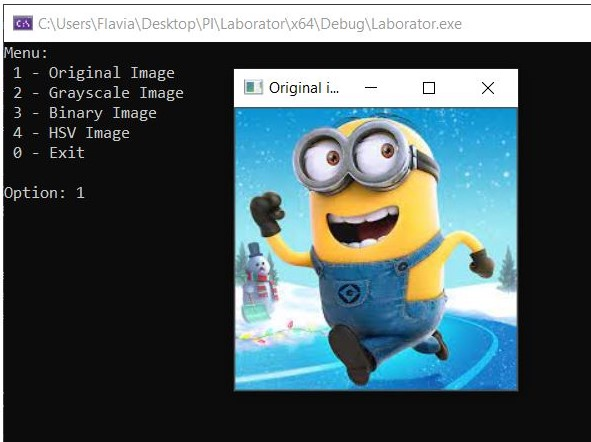
\includegraphics[width=9cm]{lab1.jpg}
\caption{Interfața corespunzătoare}
\label{fig1}
\end{figure}

\newpage

\section{Laboratorul 2}

\subsection{Descrierea aplicației}
\par
Laboratorul cu numarul 2 se referă la conversia unei imagini.
\\ \par
Pentru realizarea programului se implementează funcția grayscale\_image(), care ulterior este apelată din main de către utilizator, atunci când alege opțiunea cu numărul doi. Imaginea este citită din fișier folosind imread, cu cel de-al doilea parametru setat pe IMREAD\_GRAYSCALE, după care o afișează și o salvează pe disc cu numele GrayscaleImg.jpg.
\\ \par
Funcția binary\_image() citește o imagine din fișier folosind imread, cu cel de-al doilea parametru setat pe IMREAD\_GRAYSCALE și o convertește în binar folosind funcția \\ threshold(imaginea\_citită, imaginea\_destinație, 128, 255, THRESH\_BINARY), după care o afișează și o salvează pe disc cu numele BinaryImg.jpg.
\\ \par
Funcția hsv\_image() citește o imagine color din fișier folosind imread și o convertește în HSV folosind funcția\\cvtColor(imaginea\_citită, imaginea\_destinație, COLOR\_BGR2HSV), după care o afișează și o salvează pe disc cu numele HSVImg.jpg.

\subsection{Cod \^{i}n C++}

Codul corespunzător laboratorului 2.

\begin{lstlisting}[language=C++]{Name=lab2.c}
void grayscale_image() {
	// Citirea imaginii dintr-un fisier
	Mat img = imread("./minions.jpg", IMREAD_GRAYSCALE);
	// Vizualizarea imaginii modificate
	imshow("Grayscale image", img);
	// Salvarea imaginii modificate pe disc 
	imwrite("GrayscaleImg.jpg", img);
	waitKey(0);

}

void binary_image() {
	// Citirea imaginii dintr-un fisier
	Mat img = imread("./minions.jpg", IMREAD_GRAYSCALE);
	Mat img2;
	threshold(img, img2, 128, 255, THRESH_BINARY);

	// Vizualizarea imaginii modificate
	imshow("Binary image", img2);
	// Salvarea imaginii modificate pe disc 
	imwrite("BinaryImg.jpg", img2);
	waitKey(0);

}

void hsv_image() {
	// Citirea imaginii dintr-un fisier
	Mat img = imread("./minions.jpg");
	Mat img2;
	cvtColor(img, img2, COLOR_BGR2HSV);

	// Vizualizarea imaginii modificate
	imshow("HSV image", img2);
	// Salvarea imaginii modificate pe disc 
	imwrite("HSVImg.jpg", img2);
	waitKey(0);

}
 \end{lstlisting}

\subsection{Interfața corespunzătoare}

Rezultatul aplic\u{a}rii algoritmilor se poate observa \^{i}n figura următoare. 

\begin{figure}[ht]
\begin{tabular}{cc}
\subfloat[Imaginea original\u{a}]{
\includegraphics[width=6cm]{minions.jpg}} &
\subfloat[Grayscale]{
\includegraphics[width=6cm]{GrayscaleImg.jpg}} 
\end{tabular}
\begin{tabular}{cc}
\subfloat[Binar]{
\includegraphics[width=6cm]{BinaryImg.jpg}} &
\subfloat[HSV]{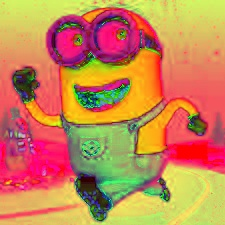
\includegraphics[width=6cm]{HSVImg.jpg}}
\end{tabular}
\caption{Imaginile prelucrate}
\end{figure}

\newpage

\section{Laboratorul 3}

\subsection{Descrierea aplicației}
\par
Laboratorul cu numarul 3 se referă la histograma unei imagini.
\\ \par
Pentru histograma unei imagini în tonuri de gri se implementează funcția \\hist\_grayscale(), care ulterior este apelată din main de către utilizator, atunci când alege opțiunea cu numărul cinci. Imaginea este citită din fișier folosind imread, cu cel de-al doilea parametru setat pe IMREAD\_GRAYSCALE (zero), iar histograma este calculată, desenată, afișată și salvată pe disc cu numele HistGrayscale.jpg.
\\ \par
Funcția color\_quantization() aplică algoritmul pragurilor multiple (cunatizarea). Aceasta citește o imagine color din fișier folosind imread, după care procesează și modifică fiecare pixel, afișează imaginea modificată și o salvează pe disc cu numele QuantizedImg.jpg.
\\ \par
Funcția Floyd\_Steinberg() aplică algoritmul de corecție Floyd-Steinberg. Funcția citește o imagine în tonuri de gri, procesează și modifică fiecare pixel și o afișează și o salvează pe disc cu numele Floyd.jpg.
\\ \par
Funcția hist\_color() calculează histograma unei imagini color. Aceasta este asemănătoare cu funcția hist\_grayscale(), dar citeste imaginea color, nu în tonuri de gri și calculează histograma pentru B, G și R. La final afișează histograma și o salvează pe disc cu numele HistColor.jpg.

\subsection{Cod \^{i}n C++}

Codul corespunzător laboratorului 3.

\begin{lstlisting}[language=C++]{Name=lab3.c}
void hist_grayscale() {

	Mat gray = imread("./minions.jpg", 0);

	// Initializarea parametrilor
	int histSize = 256;    // bin size
	float range[] = { 0, 256};
	const float* ranges[] = { range };

	// Calculul histogramei
	MatND hist;
	calcHist(&gray, 1, 0, Mat(), hist, 1, &histSize, ranges, true, false);

	// Desenarea histogramei
	int hist_w = 512;
	int hist_h = 400;
	int bin_w = cvRound((double)hist_w / histSize);

	Mat histImage(hist_h, hist_w, CV_8UC1, Scalar(0, 0, 0));
	normalize(hist, hist, 0, histImage.rows, NORM_MINMAX, -1, Mat());

	for (int i = 1; i < histSize; i++)
	{
		line(histImage, Point(bin_w * (i - 1), hist_h - cvRound(hist.at<float>(i - 1))),
			Point(bin_w * (i), hist_h - cvRound(hist.at<float>(i))),
			Scalar(255, 0, 0), 2, 8, 0);
	}

	// Vizualizarea imaginii grayscale
	imshow("Grayscale", gray);

	// Vizualizarea histogramei
	imshow("Histograma", histImage);

	// Salvarea histogramei pe disc 
	imwrite("HistGrayscale.jpg", histImage);

	waitKey(0);
}

void color_quantization() {

	Mat image = imread("./minions.jpg");

	int div = 64;

	int nl = image.rows; // Numar de linii
	int nc = image.cols * image.channels(); // Numar de elemente per linie


	for (int j = 0; j < nl; j++)
	{
		// Adresa randului j
		uchar* data = image.ptr<uchar>(j);

		for (int i = 0; i < nc; i++)
		{
			// Procesarea fiecarui pixel
			data[i] = data[i] / div * div + div / 2;
			
		}
	}

	// Vizualizarea imaginii modificate
	imshow("Cuantizare", image);
	// Salvarea imaginii modificate pe disc 
	imwrite("QuantizedImg.jpg", image);

	waitKey(0);
}

void Floyd_Steinberg() {

	Mat image = imread("./minions.jpg",IMREAD_GRAYSCALE);

	int Height = image.rows; // Numar de linii
	int Width = image.cols * image.channels(); // Numar de elemente per linie

	int old_value, new_value, Error;
	for (int y = 0; y < Height-1; y++)
	{
		// Adresa randului j
		uchar* data = image.ptr<uchar>(y);

		for (int x = 0; x < Width; x++)
		{
			// Procesarea fiecarui pixel
			old_value = data[x];
			if (old_value > 128)
				new_value = 255;
			else
				new_value = 0;
			data[x] = new_value;
			Error = old_value - new_value;

			uchar* data2 = image.ptr<uchar>(y+1);
			
			data[x + 1] +=  Error * 7 / 16;
			data2[x - 1] +=  Error * 3 / 16;
			data2[x] += Error * 5 / 16;
			data2[x + 2] += Error / 16;
		}
	}
	// Vizualizarea imaginii modificate
	imshow("Floyd Steinberg", image);
	// Salvarea imaginii modificate pe disc 
	imwrite("Floyd.jpg", image);
	waitKey(0);
}

void hist_color() {

	Mat image;

	image = imread("./minions.jpg", IMREAD_COLOR);

	if (image.empty())
	{
		return;
	}

	vector<Mat> bgr_planes;
	split(image, bgr_planes);

	int histSize = 256;

	float range[] = { 0, 256 };
	const float* histRange = { range };

	bool uniform = true;
	bool accumulate = false;

	Mat b_hist, g_hist, r_hist;

	calcHist(&bgr_planes[0], 1, 0, Mat(), b_hist, 1, &histSize, &histRange, uniform, accumulate);
	calcHist(&bgr_planes[1], 1, 0, Mat(), g_hist, 1, &histSize, &histRange, uniform, accumulate);
	calcHist(&bgr_planes[2], 1, 0, Mat(), r_hist, 1, &histSize, &histRange, uniform, accumulate);

	// Desenam histograma pentru B, G si R
	int hist_w = 512; int hist_h = 400;
	int bin_w = cvRound((double)hist_w / histSize);

	Mat histImage(hist_h, hist_w, CV_8UC3, Scalar(0, 0, 0));

	normalize(b_hist, b_hist, 0, histImage.rows, NORM_MINMAX, -1, Mat());
	normalize(g_hist, g_hist, 0, histImage.rows, NORM_MINMAX, -1, Mat());
	normalize(r_hist, r_hist, 0, histImage.rows, NORM_MINMAX, -1, Mat());

	for (int i = 1; i < histSize; i++)
	{
		line(histImage, Point(bin_w * (i - 1), hist_h - cvRound(b_hist.at<float>(i - 1))),
			Point(bin_w * (i), hist_h - cvRound(b_hist.at<float>(i))),
			Scalar(255, 0, 0), 2, 8, 0);
		line(histImage, Point(bin_w * (i - 1), hist_h - cvRound(g_hist.at<float>(i - 1))),
			Point(bin_w * (i), hist_h - cvRound(g_hist.at<float>(i))),
			Scalar(0, 255, 0), 2, 8, 0);
		line(histImage, Point(bin_w * (i - 1), hist_h - cvRound(r_hist.at<float>(i - 1))),
			Point(bin_w * (i), hist_h - cvRound(r_hist.at<float>(i))),
			Scalar(0, 0, 255), 2, 8, 0);
	}

	// Vizualizarea imaginii grayscale
	imshow("Original", image);

	// Vizualizarea histogramei
	namedWindow("Histograma Color", WINDOW_AUTOSIZE);
	imshow("Histograma Color", histImage);

	// Salvarea histogramei pe disc 
	imwrite("HistColor.jpg", histImage);

	waitKey(0);
}
 \end{lstlisting}

\subsection{Interfața corespunzătoare}

Rezultatul aplic\u{a}rii algoritmilor se poate observa \^{i}n figura următoare. 

\begin{figure}[ht]
\centering
\begin{tabular}{cc}
\subfloat[Grayscale]{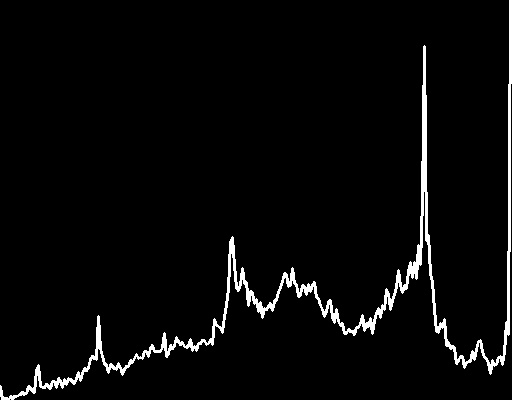
\includegraphics[width=6cm]{HistGrayscale.jpg}} &
\subfloat[Color]{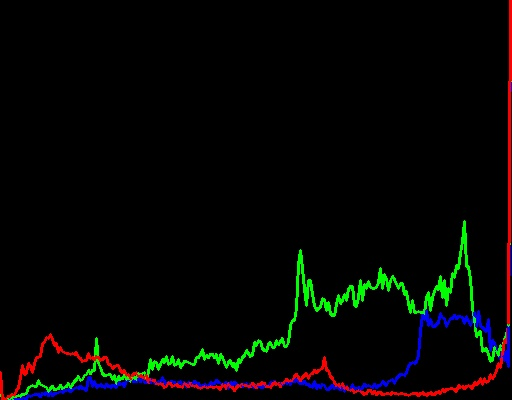
\includegraphics[width=6cm]{HistColor.jpg}} 
\end{tabular}
\caption{Histograme}
\end{figure}

\begin{figure}[ht]
\begin{tabular}{cc}
\subfloat[Algoritmul pragurilor multiple]{
\includegraphics[width=6cm]{QuantizedImg.jpg}} &
\subfloat[Algoritmul de corecție Floyd-Steinberg]{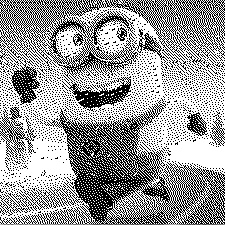
\includegraphics[width=6cm]{Floyd.jpg}} 
\end{tabular}
\caption{Algoritmii}
\end{figure}

\newpage

\section{Laboratorul 4}

\subsection{Descrierea aplicației}
\par
Laboratorul cu numarul 4 se referă la etichetarea componentelor conexe.
\\ \par
Pentru etichetarea componentelor conexe din imagini binare folosind algoritmul de traversare în lățime se implementează funcția traversare\_latime(), care ulterior este apelată din main de către utilizator, atunci când alege opțiunea cu numărul nouă. Imaginea este citită din fișier sub forma binară, precum s-a implementat functia binary\_image in cel de-al doilea laborator, după care se parcurge fiecare pixel și se modifică culoarea într-una random pentru grupurile de pixeli alaturați. Imaginea este apoi afișată și salvată pe disc cu numele bfs.jpg.
\\ \par
Funcția clase\_echivalenta() aplică algoritmul care realizează două treceri cu clase de echivalență. Aceasta citește o imagine în tonuri de gri din fișier, după care procesează și modifică fiecare pixel, asemănător cu algoritmul prezentat mai sus, afișează imaginea modificată și o salvează pe disc cu numele clsEchiv.jpg.


\subsection{Cod \^{i}n C++}

Codul corespunzător laboratorului 4.

\begin{lstlisting}[language=C++]{Name=lab3.c}
void traversare_latime() {
	int threshval = 113;
	Mat image = imread("./minions.jpg", IMREAD_GRAYSCALE);
	Mat img; threshold(image, img, 128, 255, THRESH_BINARY);
	Mat bw = threshval < 128 ? (img < threshval) : (img > threshval);
	Mat labelImage(img.size(), CV_32S);
	int nLabels = connectedComponents(bw, labelImage, 8);
	vector<Vec3b> colors(nLabels);
	colors[0] = Vec3b(0, 0, 0);

	for (int label = 1; label < nLabels; ++label) {
		colors[label] = Vec3b((rand() & 255), (rand() & 255), (rand() & 255));
	}
	Mat dst(img.size(), CV_8UC3);
	for (int r = 0; r < dst.rows; ++r) {
		for (int c = 0; c < dst.cols; ++c) {
			int label = labelImage.at<int>(r, c);
			Vec3b& pixel = dst.at<Vec3b>(r, c);
			pixel = colors[label];
		}
	}

	// Vizualizarea imaginii modificate
	imshow("Traversare latime", dst);
	// Salvarea imaginii modificate pe disc 
	imwrite("bfs.jpg", dst);
	waitKey(0);
}

void clase_echivalenta() {
	int threshval = 113;
	Mat img = imread("./minions.jpg", IMREAD_GRAYSCALE);

	Mat bw = threshval < 128 ? (img < threshval) : (img > threshval);
	Mat labelImage(img.size(), CV_32S);

	int nLabels = connectedComponents(bw, labelImage, 8);
	vector<Vec3b> colors(nLabels);
	colors[0] = Vec3b(0, 0, 0);
	for (int label = 1; label < nLabels; ++label) {
		colors[label] = Vec3b((rand() & 255), (rand() & 255), (rand() & 255));
	}
	Mat dst(img.size(), CV_8UC3);
	for (int r = 0; r < dst.rows; ++r) {
		for (int c = 0; c < dst.cols; ++c) {
			int label = labelImage.at<int>(r, c);
			Vec3b& pixel = dst.at<Vec3b>(r, c);
			pixel = colors[label];
		}
	}
	// Vizualizarea imaginii modificate
	imshow("Clase echivalente", dst);
	// Salvarea imaginii modificate pe disc 
	imwrite("clsEchiv.jpg", dst);

	waitKey(0);
}
 \end{lstlisting}

\subsection{Interfața corespunzătoare}

Rezultatul aplic\u{a}rii algoritmilor se poate observa \^{i}n figura următoare. 

\begin{figure}[ht]
\centering
\begin{tabular}{cc}
\subfloat[Algoritmul de traversare în lățime]{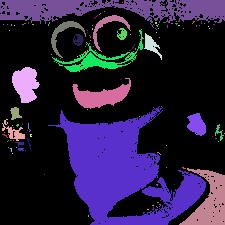
\includegraphics[width=6cm]{bfs.jpg}} &
\subfloat[Algoritmul cu clase de echivalență]{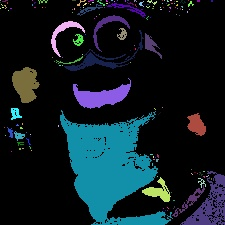
\includegraphics[width=6cm]{clsEchiv.jpg}} 
\end{tabular}
\caption{Etichetarea componentelor conexe}
\end{figure}

\newpage

\section{Laboratorul 5}

\subsection{Descrierea aplicației}
\par
Laboratorul cu numarul 5 se referă la trăsăturile geometrice ale obiectelor binare.
\\ \par
Funcția forme\_geom() citește o imagine, aplică altgoritmul prezentat la laboratorul exterior și detectează diferite forme geometrice, afișând tipul acestora și colorându-le diferit. Explicațiile detaliate se pot observa în cod, sub forma de comentarii.
\\ \par
De asemenea, avem nevoie de două funcții ajutătoare pentru realizarea acestui algoritm. Funcția angle calculeaza cosinusul unui unghi, informație care ne ajută la stabilirea formei geometrice cu 4 laturi, iar funcția setLabel ne ajută să poziționăm labelul în centrul formei geometrice cu font, dimensiune etc prestabilite.

\subsection{Cod \^{i}n C++}

Codul corespunzător laboratorului 5

\begin{lstlisting}[language=C++]{Name=lab5.c}
// Functie ajutatoare pentru gasirea cosinusului unui unghi - pt0->pt1 si pt0->pt2
static double angle(Point pt1, Point pt2, Point pt0)
{
	double dx1 = pt1.x - pt0.x;
	double dy1 = pt1.y - pt0.y;
	double dx2 = pt2.x - pt0.x;
	double dy2 = pt2.y - pt0.y;
	return (dx1 * dx2 + dy1 * dy2) / sqrt((dx1 * dx1 + dy1 * dy1) * (dx2 * dx2 + dy2 * dy2) + 1e-10);
}

// Functie ajutatoare pentru afisarea labelului in centrul unei forme geometrice
void setLabel(Mat& im, const string label, vector<Point>& contour)
{
	int fontface = FONT_HERSHEY_SIMPLEX;
	double scale = 0.4;
	int thickness = 1;
	int baseline = 0;

	Size text = getTextSize(label, fontface, scale, thickness, &baseline);
	Rect r = boundingRect(contour);

	Point pt(r.x + ((r.width - text.width) / 2), r.y + ((r.height + text.height) / 2));
	putText(im, label, pt, fontface, scale, CV_RGB(0, 0, 0), thickness, 8);
}
void forme_geom(){
	Mat img = imread("./shapes.jpg");
	Mat gray, bw;
	vector<vector<Point> > contours;
	vector<Point> approx;

	imshow("Orginal image", img);

	// Convertim imaginea in grayscale si o salvam in grey
	cvtColor(img, gray, COLOR_BGR2GRAY);

	// Salvam in bw imaginea grayscale cu algoritmul Canny aplicat
	blur(gray, bw, Size(3, 3));
	Canny(gray, bw, 80, 240, 3);

	// Gasim contururile
	findContours(bw.clone(), contours, RETR_EXTERNAL, CHAIN_APPROX_SIMPLE);

	for (int i = 0; i < contours.size(); i++)
	{
		// Aproximam conturul cu o acuratete de 0.02
		approxPolyDP(Mat(contours[i]), approx, arcLength(Mat(contours[i]), true) * 0.02, true);

		// Sarim peste obiectele mici sau non-convexe
		if (fabs(contourArea(contours[i])) < 100 || !isContourConvex(approx))
			continue;
		if (approx.size() == 3)
		{
			drawContours(img, contours, i, Scalar(244, 232, 193), FILLED);
			setLabel(img, "Triunghi", contours[i]);
		}
		else if (approx.size() >= 4 && approx.size() <= 6)
		{
			// Calculam numarul de laturi
			int vtc = approx.size();

			// Calculam cosinusurile colturilor
			vector<double> cos;
			for (int j = 2; j < vtc + 1; j++)
				cos.push_back(angle(approx[j % vtc], approx[j - 2], approx[j - 1]));

			sort(cos.begin(), cos.end());
			double mincos = cos.front();
			double maxcos = cos.back();

			// Decidem ce forma geometrica este si o coloram corespunzator
			if (vtc == 4) {
				drawContours(img, contours, i, Scalar(160, 193, 185), FILLED);
				setLabel(img, "Dreptunghi", contours[i]);
			}
			else if (vtc == 5) {
				drawContours(img, contours, i, Scalar(112, 160, 175), FILLED);
				setLabel(img, "Pentagon", contours[i]);
			}
			else if (vtc == 6) {
				drawContours(img, contours, i, Scalar(112, 105, 147), FILLED);
				setLabel(img, "Hexagon", contours[i]);
			}
		}
		else
		{
			// Detectam si coloram cercurile
			double area = contourArea(contours[i]);
			Rect r = boundingRect(contours[i]);
			int radius = r.width / 2;

			if (abs(1 - ((double)r.width / r.height)) <= 0.2 &&
				abs(1 - (area / (CV_PI * (radius * radius)))) <= 0.2)
				drawContours(img, contours, i, Scalar(181, 146, 160), FILLED);
			setLabel(img, "Cerc", contours[i]);
		}
	}
	imshow("Modified image", img);
	imwrite("formeGeom.jpg", img);
	waitKey(0);
}
 \end{lstlisting}

\subsection{Interfața corespunzătoare}

Rezultatul aplic\u{a}rii algoritmului se poate observa \^{i}n figura următoare. 

\begin{figure}[ht]
\centering
\begin{tabular}{cc}
\subfloat[Imaginea originală]{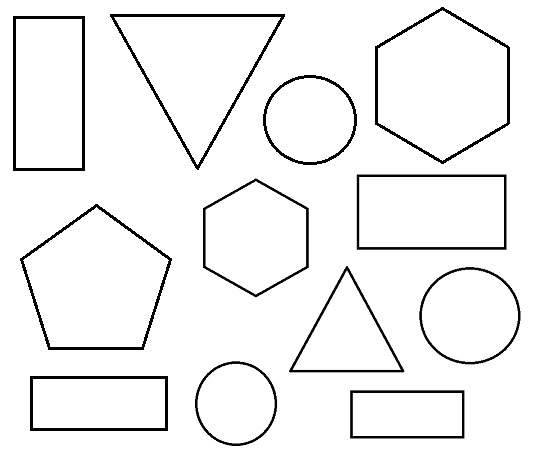
\includegraphics[width=6cm]{shapes.jpg}} &
\subfloat[Imaginea rezultată]{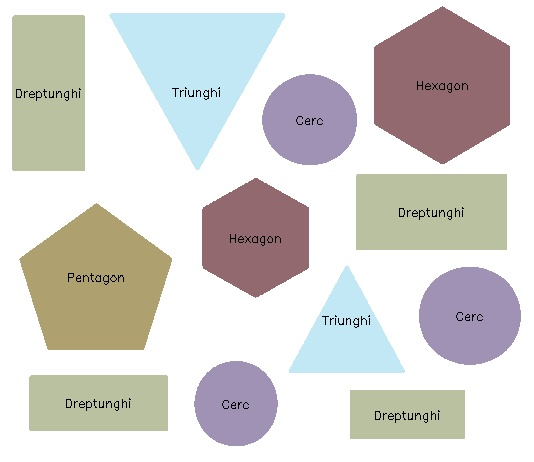
\includegraphics[width=6cm]{formeGeom.jpg}} 
\end{tabular}
\caption{Trăsăturile geometrice ale obiectelor binare}
\end{figure}

\newpage

\section{Laboratorul 6}

\subsection{Descrierea aplicației}
\par
Laboratorul cu numarul 6 se referă la extragerea conturului unui obiect dintr-o imagine.
\\ \par
Funcția tracing() citește o imagine grayscale și o convertește în binar. Imaginii binare i se aplică funcția findContours() pentru găsirea conturului, după care facem toată imaginea neagră și desenăm conturul cu alb, folosind funcția drawContours(). La final afișăm imaginea și o salvăm cu numele contur.jpg.

\subsection{Cod \^{i}n C++}

Codul corespunzător laboratorului 6

\begin{lstlisting}[language=C++]{Name=lab5.c}
void tracing() {
	Mat g_gray, g_binary;
	//Citim imaginea grayscale
	g_gray = imread("./minions.jpg", 0);
	//Salvam in g_binary imaginea binara
	threshold(g_gray, g_binary, 100, 255, THRESH_BINARY);
	//Gasim conturul
	vector< vector< Point> > contours;
	findContours(g_binary, contours, noArray(), RETR_LIST, CHAIN_APPROX_SIMPLE);
	//Facem toata poza neagra
	g_binary = Scalar::all(0);
	//Desemnam conturul cu alb
	drawContours(g_binary, contours, -1, Scalar::all(255));
	//Afisam si salvam imaginea
	imshow("Contur", g_binary);
	imwrite("contur.jpg", g_binary);
	waitKey(0);
}
 \end{lstlisting}

\subsection{Interfața corespunzătoare}

Rezultatul aplic\u{a}rii algoritmului se poate observa \^{i}n figura următoare. 
\begin{figure}[ht]
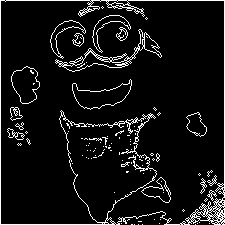
\includegraphics[width=6cm]{contur.jpg}
\caption{Extragerea conturului unui obiect dintr-o imagine}
\end{figure}


\newpage

\section{Laboratorul 7}

\subsection{Descrierea aplicației}
\par
Laboratorul cu numarul 7 se referă la operațiile morfologice pe imagini binare.
\\ \par
Funcția deschidere() citește o imagine căreia îi aplică eroziunea, după care imaginii rezultate îi aplică dilatarea. La final afișăm imaginea finală și o salvăm cu numele deschidere.jpg.
\\ \par
Funcția inchidere() citește o imagine căreia îi aplică dilatarea, după care imaginii rezultate îi aplică eroziunea. La final afișăm imaginea finală și o salvăm cu numele inchidere.jpg.
\\ \par
Funcția extragere() citește o imagine și o salvează convertită în grayscale. Se aplică funcția morphologyEx() cu cel de-al treilea paramentru, și anume operația, setat pe MORPH\_TOPHAT. Această funcție scade din imaginea originală deschiderea acesteia. La final afișăm imaginea rezultată și o salvăm cu numele extragere.jpg.
\\ \par
Funcția umplere() citește o imagine și o salvează convertită în grayscale. Se aplică funcția morphologyEx() cu cel de-al treilea paramentru, și anume operația, setat pe MORPH\_BLACKHAT. Această funcție scade din ănchiderea unei imagini imaginea în sine. La final afișăm imaginea rezultată și o salvăm cu numele umplere.jpg.
\\ \par

\subsection{Cod \^{i}n C++}

Codul corespunzător laboratorului 7

\begin{lstlisting}[language=C++]{Name=lab7.c}
void deschidere() {
	Mat erosion_dst, dilation_dst;
	Mat src = imread("./minions.jpg");

	//Aplicam eroziunea
	int erosion_size = 7;
	Mat element = getStructuringElement(MORPH_CROSS,
		Size(2 * erosion_size + 1, 2 * erosion_size + 1),
		Point(erosion_size, erosion_size));
	erode(src, erosion_dst, element);
	imshow("Eroziune", erosion_dst);
	imwrite("deschidere1.jpg", erosion_dst);
	
	//Aplicam dilatarea pe imaginea erodata
	int dilation_size = 5;
	Mat element2 = getStructuringElement(MORPH_CROSS,
		Size(2 * dilation_size + 1, 2 * dilation_size + 1),
		Point(dilation_size, dilation_size));
	dilate(erosion_dst, dilation_dst, element2);
	imshow("Deschidere", dilation_dst);
	imwrite("deschidere.jpg", dilation_dst);

	waitKey(0);

}
void inchidere() {
	Mat erosion_dst, dilation_dst;
	Mat src = imread("./minions.jpg");

	//Aplicam dilatarea
	int dilation_size = 5;
	Mat element2 = getStructuringElement(MORPH_CROSS,
		Size(2 * dilation_size + 1, 2 * dilation_size + 1),
		Point(dilation_size, dilation_size));
	dilate(src, dilation_dst, element2);
	imshow("Dilatare", dilation_dst);
	imwrite("inchidere1.jpg", dilation_dst);

	//Aplicam eroziunea pe imaginea dilatata
	int erosion_size = 7;
	Mat element = getStructuringElement(MORPH_CROSS,
		Size(2 * erosion_size + 1, 2 * erosion_size + 1),
		Point(erosion_size, erosion_size));
	erode(dilation_dst, erosion_dst, element);
	imshow("Inchidere", erosion_dst);
	imwrite("inchidere.jpg", erosion_dst);

	waitKey(0);
}
void extragere() {
	Mat src, dst, top;
	//Citim imaginea color
	src = imread("./minions.jpg");
	cvtColor(src, dst, COLOR_BGR2GRAY);
	int morph_size = 5;
	Mat element = getStructuringElement(MORPH_CROSS,
		Size(2 * morph_size + 1, 2 * morph_size + 1), Point(morph_size, morph_size));
	morphologyEx(dst, top, MORPH_TOPHAT, element);
	imshow("TopHat", top);
	imwrite("extragere.jpg", top);

	waitKey(0);
}
void umplere() {
	Mat src, dst, black;
	//Citim imaginea color
	src = imread("./minions.jpg");
	cvtColor(src, dst, COLOR_BGR2GRAY);
	int morph_size = 5;
	Mat element = getStructuringElement(MORPH_CROSS,
		Size(2 * morph_size + 1, 2 * morph_size + 1), Point(morph_size, morph_size));
	morphologyEx(dst, black, MORPH_BLACKHAT, element);
	imshow("BlackHat", black);
	imwrite("umplere.jpg", black);

	waitKey(0);
}
 \end{lstlisting}

\subsection{Interfața corespunzătoare}

Rezultatul aplic\u{a}rii algoritmilor se poate observa \^{i}n figura următoare. 
\begin{figure}[ht]
\centering
\begin{tabular}{cc}
\subfloat[Deschiderea]{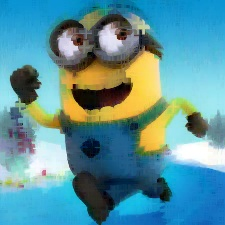
\includegraphics[width=13cm]{deschidere.jpg}} &
\end{tabular}
\begin{tabular}{cc}
\subfloat[Inchiderea]{
\includegraphics[width=13cm]{inchidere.jpg}} &
\end{tabular}
\begin{tabular}{cc}
\subfloat[Extragerea conturului]{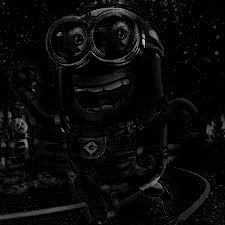
\includegraphics[width=6cm]{extragere.jpg}} &
\subfloat[Umplerea regiunilor]{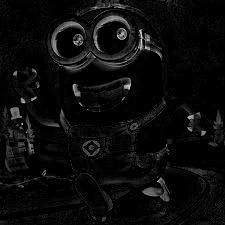
\includegraphics[width=6cm]{umplere.jpg}} 
\end{tabular}
\caption{Operații morfologice pe imagini binare}
\end{figure}

\newpage

\section{Laboratorul 8}

\subsection{Descrierea aplicației}
\par
Laboratorul cu numarul 8 se referă la proprietățile statistice ale imaginilor de intensitate.
\\ \par
Funcția seeHist() este o funcție ajutătoare, și anume funcția hist\_grayscale(), prezentată la laboratorul 3. Aceasta calculează și afișează histograma unei imagini grayscale.
\\ \par
Funcția eghist() implementează algoritmul de egalizare a histogramei, folosind funcția equalizeHist(imagineaGrayscale, imagineaDestinație). \\Atât imaginea destinație cât și histogramele sunt salvate pe disc. Imaginea cu denumirea eqImg.jpg, iar histogramele în funcție de parametrul index[] trimis.

\subsection{Cod \^{i}n C++}

Codul corespunzător laboratorului 8

\begin{lstlisting}[language=C++]{Name=lab8.c}

void seeHist(Mat gray,char index[10]) {
	// Initializarea parametrilor
	int histSize = 256;    // bin size
	float range[] = { 0, 256 };
	const float* ranges[] = { range };
	// Calculul histogramei
	MatND hist;
	calcHist(&gray, 1, 0, Mat(), hist, 1, &histSize, ranges, true, false);
	// Desenarea histogramei
	int hist_w = 512;
	int hist_h = 400;
	int bin_w = cvRound((double)hist_w / histSize);
	Mat histImage(hist_h, hist_w, CV_8UC1, Scalar(0, 0, 0));
	normalize(hist, hist, 0, histImage.rows, NORM_MINMAX, -1, Mat());
	for (int i = 1; i < histSize; i++)
	{
		line(histImage, Point(bin_w * (i - 1), hist_h - cvRound(hist.at<float>(i - 1))),
			Point(bin_w * (i), hist_h - cvRound(hist.at<float>(i))),
			Scalar(255, 0, 0), 2, 8, 0);
	}
	// Vizualizarea histogramei
	imshow("Histograma", histImage);
	char s[20] = "hist";
	strcat_s(s, index);
	strcat_s(s, ".jpg\0");
	// Salvarea histogramei pe disc 
	imwrite(s, histImage);
	waitKey(0);
}
void eghist() {
	Mat src = imread("./minions.jpg",0);
	Mat dst;
	char s[10];
	equalizeHist(src, dst);
	imshow("Source image", src);
	strcpy_s(s,"Orig");
	seeHist(src,s);
	imshow("Equalized Image", dst);
	imwrite("eqImg.jpg", dst);
	strcpy_s(s, "Rez");
	seeHist(dst, s);
	waitKey(0);
}
 \end{lstlisting}

\subsection{Interfața corespunzătoare}

Rezultatul aplic\u{a}rii algoritmului se poate observa \^{i}n figura următoare. 
\begin{figure}[ht]
\centering
\begin{tabular}{cc}
\subfloat[Imaginea originală]{
\includegraphics[width=5cm]{GrayscaleImg.jpg}} &
\subfloat[Histograma ei]{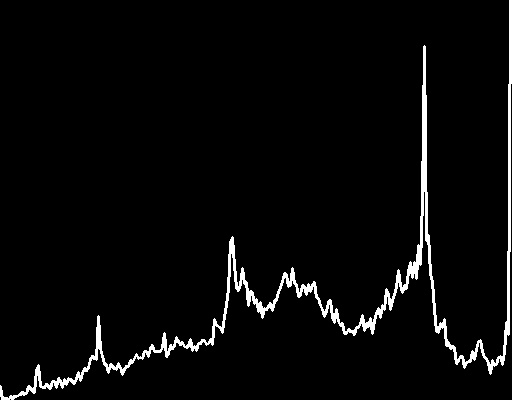
\includegraphics[width=6.5cm]{histOrig.jpg}}
\end{tabular}
\begin{tabular}{cc}
\subfloat[Imaginea egalizată]{
\includegraphics[width=5cm]{eqImg.jpg}} &
\subfloat[Histograma ei]{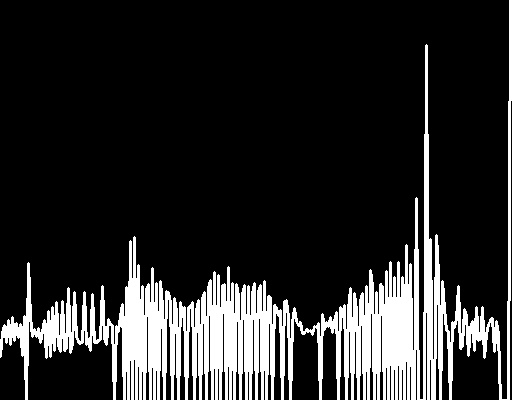
\includegraphics[width=6.5cm]{histRez.jpg}}
\end{tabular}
\caption{Proprietăți statistice ale imaginilor de intensitate
}
\end{figure}

\newpage

\section{Laboratorul 9}

\subsection{Descrierea aplicației}
\par
Laboratorul cu numarul 9 se referă la filtrarea imaginilor în domeniul spațial.
\\ \par
Funcția lowpass() implementează filtrul gausian de tip „trece-jos”. Aceasta citește imaginea grayscale și, folosind funcția predefinită GaussianBlur, cu kernel de dimensiune 5x5, salvează poza modificată în variabila lowp, după care o afișează și o salvează pe disc cu numele lowpass.jpg.
\\ \par
Funcția highpass() implementează filtrul gausian de tip „trece-sus”. Aceasta citește imaginea grayscale și, folosind funcția predefinită GaussianBlur, cu kernel de dimensiune 11x11, salvează poza blurată în variabila blur, după care se salvează în variabila highp imaginea finală, formată din diferența dintre imaginea inițială și cea blurată. La final afișează imaginea highp și o salvează pe disc cu numele highpass.jpg.

\subsection{Cod \^{i}n C++}

Codul corespunzător laboratorului 9

\begin{lstlisting}[language=C++]{Name=lab9.c}

void lowpass() {
	Mat img = imread("./minions.jpg", 0);
	Mat lowp;

	GaussianBlur(img, lowp, Size(5, 5), 0, 0, BORDER_DEFAULT);

	imshow("LowPass", lowp);
	imwrite("lowpass.jpg", lowp);

	waitKey(0);
}
void highpass() {
	Mat img = imread("./minions.jpg", 0);
	Mat blur,highp;

	GaussianBlur(img, blur, Size(11, 11), 0, 0, BORDER_DEFAULT);

	highp = img - blur;

	imshow("HighPass", highp);
	imwrite("highpass.jpg", highp);

	waitKey(0);
}

 \end{lstlisting}

\subsection{Interfața corespunzătoare}

Rezultatul aplic\u{a}rii algoritmului se poate observa \^{i}n figura următoare. 

\begin{figure}[ht]
\centering
\begin{tabular}{cc}
\subfloat[Trece-sus]{
\includegraphics[width=6cm]{lowpass.jpg}} &
\subfloat[Trece-jos]{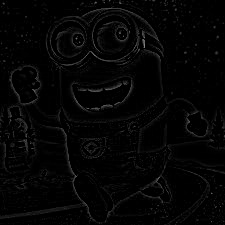
\includegraphics[width=6cm]{highpass.jpg}}
\end{tabular}
\caption{Filtrarea imaginilor în domeniul spațial}
\end{figure}


\newpage

\section{Laboratorul 10}

\subsection{Descrierea aplicației}
\par
Laboratorul cu numarul 10 se referă la filtrarea imaginilor în domeniul frecvențial.
\\ \par
Funcția fourier() implementează Transformata Fourier discretă (DFT). Aceasta citește imaginea grayscale, o divizează în două canale, și anume în partea reală și în cea imaginară, după care calculează magnitudinea imaginii, o centralizează, normalizează și afișează rezultatul.
\\ \par
Funcția gauss() implementează filtrul gausian de tip „trece-jos”. Aceasta citește imaginea grayscale și, folosind funcția predefinită GaussianBlur, cu sigma de dimensiune 45, modifică imaginea și o salvează în variabila gaussianBlur, după care o normalizează și o afișează.

\subsection{Cod \^{i}n C++}

Codul corespunzător laboratorului 10

\begin{lstlisting}[language=C++]{Name=lab10.c}

void fourier() {

	// Citim imaginea grayscale
	Mat src = imread("./minions.jpg", 0);

	// Divizarea in doua canale: partea reala si partea imaginara
	Mat channels[] = { Mat_<float>(src), Mat::zeros(src.size(), CV_32F) };
	Mat complexI;
	merge(channels, 2, complexI); 
	dft(complexI, complexI);
	split(complexI, channels);

	// Calcularea magnitudinii cu elemente de tip float
	Mat magSrc;
	magnitude(channels[0], channels[1], magSrc);
	magSrc += Scalar::all(1);
	log(magSrc, magSrc);

	// Centralizarea imaginii
	int cx = magSrc.cols / 2;
	int cy = magSrc.rows / 2;
	Mat q0(magSrc, Rect(0, 0, cx, cy));   // Stanga-Sus
	Mat q1(magSrc, Rect(cx, 0, cx, cy));  // Dreapta-Sus
	Mat q2(magSrc, Rect(0, cy, cx, cy));  // Stanga-Jos
	Mat q3(magSrc, Rect(cx, cy, cx, cy)); // Dreapta-Jos
	
	Mat tmp;
	// Inversam stanga-sus cu dreapta-jos
	q0.copyTo(tmp);
	q3.copyTo(q0);
	tmp.copyTo(q3);
	q1.copyTo(tmp);
	// Inversam dreapta-sus cu stanga-jos
	q2.copyTo(q1);
	tmp.copyTo(q2);
	// Normalizam rezultatul in imaginea destinatie
	normalize(magSrc, magSrc, 0, 1, NORM_MINMAX);		

	//Afisarea pozei originale si a rezultatului
	imshow("Originala", src);
	imshow("DFT", magSrc);
	//imwrite("dft.jpg", magSrc);

	waitKey(0);
}
void gauss() {

	// Citim imaginea grayscale
	Mat src = imread("./minions.jpg", 0);

	// Salvam in srcf imaginea convertita in float (CV_32FC1)
	Mat srcf;
	src.convertTo(srcf, CV_32FC1);

	// Aplicam estomparea Gaussiana
	Mat gaussianBlur(src.size(), CV_32FC1);
	float sigma = 45;
	float d0 = 2 * sigma * sigma;
	for (int i = 0; i < srcf.rows; i++)
	{
		for (int j = 0; j < srcf.cols; j++)
		{
			float d = pow(float(i - srcf.rows / 2), 2) + pow(float(j - srcf.cols / 2), 2);
			gaussianBlur.at<float>(i, j) = expf(-d / d0);
		}
	}

	// Normalizam rezultatul in imaginea destinatie
	normalize(gaussianBlur, gaussianBlur, 0, 1, NORM_MINMAX);
	imshow("Gauss", gaussianBlur);
	//imwrite("gauss.jpg", gaussianBlur);

	waitKey(0);
}
 \end{lstlisting}

\subsection{Interfața corespunzătoare}

Rezultatul aplic\u{a}rii algoritmilor se poate observa \^{i}n figura următoare. 
\begin{figure}[ht]
\centering
\begin{tabular}{cc}
\subfloat[DFT]{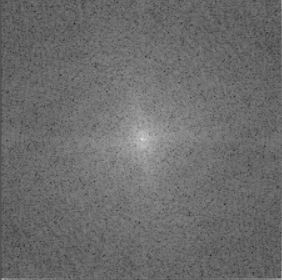
\includegraphics[width=6cm]{dft.jpg}} &
\subfloat[Gaussian Trece-jos]{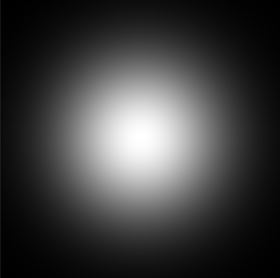
\includegraphics[width=6cm]{gauss.jpg}}
\end{tabular}

\caption{Filtrarea imaginilor în domeniul frecvențial}
\end{figure}

\newpage
\section{Laboratorul 11}

\subsection{Descrierea aplicației}
\par
Laboratorul cu numarul 11 se referă la eliminarea zgomotelor din imagnile digitale.
\\ \par
Funcția nucleugauss() implementează algoritmul de filtrare/restaurare a unei imagni prin convoluția acesteia cu un nucleu gaussian. Aceasta citește imaginea color, o salvează în variabila dst după aplicarea funcției cv.GaussianBlur, iar la final o afișează și o salvează pe disc cu numele nucleugauss.jpg.
\\ \par
Funcția nucleubi() implementează algoritmul de filtrare/restaurare a unei imagni prin convoluția acesteia cu un nucleu bidimensional. Aceasta citește imaginea color, o modifică în grayscale, o salvează în variabila dst după aplicarea funcției cv.bilateralFilter, iar la final o afișează și o salvează pe disc cu numele nucleubi.jpg.
\\ \par
De asemenea, ambele funcții calculează și afișează și timpul de procesare.

\subsection{Cod \^{i}n C++}

Codul corespunzător laboratorului 11

\begin{lstlisting}[language=C++]{Name=lab11.c}
void nucleugauss() {

	//Timp de procesare
	clock_t begin = clock();
	// Citim imaginea
	Mat src = imread("./noise.jpg");
	imshow("Originala", src);
	// Salvam in dst imaginea convertita
	Mat dst;
	Size ksize = Size(3, 3);
	GaussianBlur(src, dst, ksize, 100, 100, BORDER_DEFAULT);
	// Afisam si salvam imaginea convertita
	imshow("Nucleu Gauss", dst);
	imwrite("nucleugauss.jpg", dst);
	//Timp de procesare
	clock_t end = clock();
	double diffticks = end - begin;
	double diffms = (diffticks * 1000) / CLOCKS_PER_SEC;
	cout << "Timpul de procesare: " << double(diffms) << " ms (" << double(diffms) / 1000 << " sec) \n\n";

	waitKey(0);
}

void nucleubi() {

	//Timp de procesare
	clock_t begin = clock();
	// Citim imaginea
	Mat src = imread("./noise.jpg");
	imshow("Originala", src);
	cvtColor(src, src, COLOR_RGBA2RGB, 0);
	// Salvam in dst imaginea convertita
	Mat dst;
	bilateralFilter(src, dst, 9, 100, 100, BORDER_DEFAULT);
	// Afisam si salvam imaginea convertita
	imshow("Nucleu Bidimensional", dst);
	imwrite("nucleubi.jpg", dst);
	//Timp de procesare
	clock_t end = clock();
	double diffticks = end - begin;
	double diffms = (diffticks * 1000) / CLOCKS_PER_SEC;
	cout << "Timpul de procesare: " << double(diffms) << " ms (" << double(diffms) / 1000 << " sec) \n\n";

	waitKey(0);
}
 \end{lstlisting}

\subsection{Interfața corespunzătoare}

Rezultatul aplic\u{a}rii algoritmilor se poate observa \^{i}n figura următoare. 
\begin{figure}[ht]
\centering
\begin{tabular}{cc}
\subfloat[Originala]{
\includegraphics[width=5cm]{noise.jpg}} &
\subfloat[Nucleu Gaussian]{
\includegraphics[width=5cm]{nucleugauss.jpg}}
\end{tabular}
\begin{tabular}{cc}
\subfloat[Nucleu bidimensional]{
\includegraphics[width=5cm]{nucleubi.jpg}} &
\subfloat[Timp de procesare]{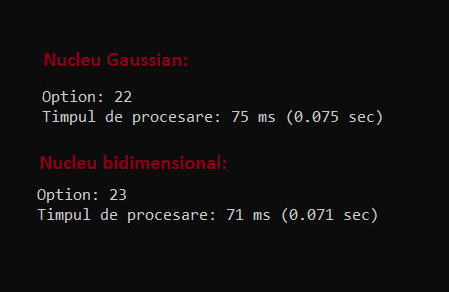
\includegraphics[width=7.7cm]{tp.png}}
\end{tabular}
\caption{Eliminarea zgomotelor din imaginile digitale}
\end{figure}


\newpage
\section{Laboratorul 12}

\subsection{Descrierea aplicației}
\par
Laboratorul cu numarul 12 se referă la detecția punctelor de muchie.
\\ \par
Funcția binadapt() implementează algoritmul de binarizare adaptivă a punctelor de muchie. Aceasta citește imaginea grayscale, o salvează în variabila dst după aplicarea funcției cv.adaptiveThreshold, iar la final o afișează și o salvează pe disc cu numele binadapt.jpg.
\\ \par
Funcția histereza() implementează algoritmul de prelungire a muchiilor prin histereză. Aceasta citește imaginea color, o modifică în grayscale, o blurează, ii aplică funcția Canny, iar la final copiază în variabila dst (imagine all black) doar muchiile, o afișează și o salvează pe disc cu numele histereza.jpg.

\subsection{Cod \^{i}n C++}

Codul corespunzător laboratorului 12

\begin{lstlisting}[language=C++]{Name=lab12.c}
void binadapt() {

	// Citim imaginea grayscale
	Mat src = imread("./minions.jpg",0);
	// Salvam in dst imaginea convertita
	Mat dst;
	adaptiveThreshold(src, dst, 200, ADAPTIVE_THRESH_GAUSSIAN_C, THRESH_BINARY, 3, 2);
	// Afisam si salvam imaginea convertita
	imshow("Binarizare adaptiva", dst);
	imwrite("binadapt.jpg", dst);

	waitKey(0);
}
void histereza() {

	// Citim imaginea
	Mat src = imread("./minions.jpg");
	Mat gray,edges,dst;
	// Convertim imaginea in grayscale
	cvtColor(src, gray, COLOR_BGR2GRAY);
	// Bluram imaginea grayscale cu un kernel de dimensiune 3
	blur(gray, edges, Size(3, 3));
	// Aplicam functia Canny
	Canny(edges, edges, 60, 60 * 3);
	// Facem ca dst sa fie toata neagra si copiem doar muchiile
	dst = Scalar::all(0);
	src.copyTo(dst, edges);
	// Afisam si salvam imaginea convertita
	imshow("Histereza", dst);
	imwrite("histereza.jpg", dst);

	waitKey(0);
}
 \end{lstlisting}

\subsection{Interfața corespunzătoare}

Rezultatul aplic\u{a}rii algoritmilor se poate observa \^{i}n figura următoare. 
\begin{figure}[ht]
\centering
\begin{tabular}{cc}
\subfloat[Binarizare adaptivă]{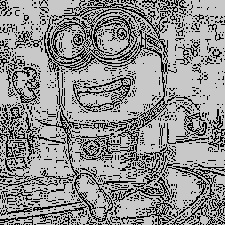
\includegraphics[width=6cm]{binadapt.jpg}} &
\subfloat[Histereză]{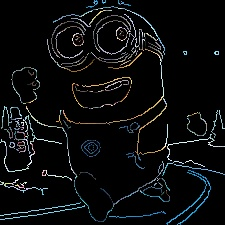
\includegraphics[width=6cm]{histereza.jpg}}
\end{tabular}

\caption{Detecția punctelor de muchie}
\end{figure}

% lucrarile incluse in bibliografie se citeaza obligatoriu in textul lucrarii
% folosind comanda \cite
\begin{thebibliography}{99}
 \bibitem{classroom} \url{https://classroom.google.com/u/1/c/MTY4MzUwODY1NzQy}
 \bibitem{carte} \textsc{Adrian Kaehler} \c{s}i \textsc{Gary Bradski}, \emph{Learning OpenCV 3 - COMPUTER VISION IN C++ WITH THE OPENCV LIBRARY}, O'REILLY, USA, 2017.
\end{thebibliography}

\end{document}